\documentclass{article}
\usepackage[margin=2.5cm, top=4cm, headheight=25pt]{geometry}
\usepackage{amsmath, amssymb, enumitem, fancyhdr, graphicx}
\usepackage[indent=20pt]{parskip}
\usepackage[hidelinks]{hyperref}
\usepackage{xcolor}
\usepackage{listings}
\usepackage{subcaption}
\usepackage{url}
\usepackage[most]{tcolorbox}
\usepackage{lastpage}
\usetikzlibrary{arrows, shapes}

\tcbuselibrary{listingsutf8} % Support for lstlistings within tcolorbox

\newtcolorbox[auto counter, number within=section]{question}[1][]{%
    colframe=gray!80,                      % Dark gray frame
    colback=gray!5,                       % Light gray background
    coltitle=black,                        % Black title
    title=\textbf{Question~\thetcbcounter}, % Bold title
    fonttitle=\bfseries\large,             % Subtle title font size
    rounded corners,                   % Slightly more rounded corners
    boxrule=0.25mm,                         % Thinner border for a sleek look
    enhanced,                              % Enhanced box features
    attach boxed title to top left={xshift=2mm, yshift=-2mm},
    boxed title style={colframe=gray!80, colback=gray!5, boxrule=0.25mm},
    % Title styling
    #1
}

\bibliographystyle{IEEEtran}
\graphicspath{{./images/}}

% -- Custom Variables --
\def\me{Rajdeep Gill 7934493}
\def\course{ECE 4260}
\def\labsection{A01}

\def\labno{3}
\def\title{Assignment 3}

% -- Styling for code snippets --
\lstset{
    basicstyle=\ttfamily\scriptsize,           % Basic font style
    keywordstyle=\color{blue},            % Keywords color
    commentstyle=\color{gray},            % Comments color
    stringstyle=\color{teal},             % Strings color
    numbers=left,                         % Line numbers on the left
    numberstyle=\tiny\color{gray},        % Line number style
    stepnumber=1,                         % Line number step
    numbersep=10pt,                       % Space between line numbers and code
    backgroundcolor=\color{lightgray!10}, % Background color
    frame=single,                         % Adds a frame around the code
    breaklines=true,                      % Line breaking for long lines
    captionpos=b,                         % Caption position
    showspaces=false,                     % Don't show spaces
    showstringspaces=false                % Don't show spaces in strings
}
\renewcommand{\lstlistingname}{Code Snippet}

\renewcommand{\arraystretch}{1.2} % For less-ugly tables
\setlength\parindent{0pt}

%----- Samples 
% Questions:
%   \begin{question}[title=Custom Question Title]
%       Question details
%   \end{question}

% Tables:
%   \begin{table}[htbp]
%       \centering
%       \caption{Table Caption}
%       \begin{tabular}{ll}
%           \toprule
%           \textbf{Column 1} & \textbf{Column 2} \\
%           \midrule
%           Row 1 & Row 2 \\
%           Row 3 & Row 4 \\
%           \bottomrule
%       \end{tabular}
%   \end{table} 

% Figures:
%   Single figure:
%       \begin{figure}[htbp]
%           \centering
%           \includegraphics[width=0.5\textwidth]{example-image}
%           \caption{Figure Caption}
%       \end{figure}
%   Multiple figures:
%       \begin{figure}[htbp]
%           \centering
%           \begin{subfigure}[b]{0.5\textwidth}
%               \includegraphics[width=\textwidth]{example-image-a}
%               \caption{First subfigure}
%           \end{subfigure}
%           \begin{subfigure}[b]{0.5\textwidth}
%               \includegraphics[width=\textwidth]{example-image-b}
%               \caption{Second subfigure}
%           \end{subfigure}
%           \caption{Main figure}
%       \end{figure}

\begin{document}

% --------------------------------------------------------------------------------
% TITLE
% --------------------------------------------------------------------------------

\begin{center}
    \huge \title

    \vspace{2mm}
    \hrule

    \vspace{4mm}
    \large \me

    \vspace{2mm}
    \large \course~\labsection

    \vspace{2mm}
    \today
\end{center}

\vspace{4mm}

% --------------------------------------------------------------------------------
% END TITLE
% --------------------------------------------------------------------------------

\newpage


\vspace{1cm}
\newpage

\pagestyle{fancy}
\fancyhead[L]{\large Assignment \labno}
\fancyhead[R]{\large \me}

\fancyfoot[C]{Page \thepage~of~\pageref{LastPage}}

% --------------------------------------------------------------------------------
% BODY
% --------------------------------------------------------------------------------
\section{Problem 1}

\begin{enumerate}[label=1.\arabic*]
    \item We can show the following:
    \begin{align*}
        \int_{-\infty}^{\infty} g_1(t)g_2^*(t) \, dt &= \int_{-\infty}^{\infty} G_1(f)G_2^*(f) \, df
    \end{align*}

    Starting with the left-hand side:
    \begin{align*}
        \int_{-\infty}^{\infty} g_1(t)g_2^*(t) \, dt &= \int_{-\infty}^{\infty} g_1(t) \left( \int_{-\infty}^{\infty} G_2^*(f)e^{-j2\pi ft} \, df \right) \, dt \\
        &= \int_{-\infty}^{\infty} G_2^*(f) \left( \int_{-\infty}^{\infty} g_1(t)e^{j2\pi ft} \, dt \right) \, df \\
        &= \int_{-\infty}^{\infty} G_2^*(f)G_1(f) \, df \\
        &= \int_{-\infty}^{\infty} G_1(f)G_2^*(f) \, df
    \end{align*}
    And thus, we have shown that the left-hand side is equal to the right-hand side.

    \item \textit{Explain how we can obtain Parseval's Theorem from (1).}
    To find Parseval's Theorem, we can set $g_1(t) = g_2(t) = g(t)$, which implies that $G_1(f) = G_2(f) = G(f)$. Substituting these values into (1.1), we get:
    \begin{align*}
        \int_{-\infty}^{\infty} g(t)g^*(t) \, dt &= \int_{-\infty}^{\infty} G(f)G^*(f) \, df \\
        \int_{-\infty}^{\infty} |g(t)|^2 \, dt &= \int_{-\infty}^{\infty} |G(f)|^2 \, df
    \end{align*}
    \item Using Parseval's Theorem, show that for any $k>0$ we have:
    \begin{align*}
        \int_{-\infty}^{\infty} \text{sinc}^2(kt) \, dt = \frac{1}{k}
    \end{align*}

    Here we have:
    \begin{align*}
        g(t) = \text{sinc}(kt), \quad G(f) = \frac{1}{k}\text{rect}\left(\frac{f}{k}\right)
    \end{align*}

    The conjugate of a rect function is itself, so we have:
    \begin{align*}
        \int_{-\infty}^{\infty} \text{sinc}^2(kt) \, dt &= \int_{-\infty}^{\infty} \frac{1}{k}\text{rect}\left(\frac{f}{k}\right)\frac{1}{k}\text{rect}\left(\frac{f}{k}\right) \, df \\
        &= \frac{1}{k^2}\int_{-k/2}^{k/2} \text{rect}\left(\frac{f}{k}\right) \, df \\
        &= \frac{1}{k^2}\int_{-k/2}^{k/2} 1 \, df \\
        &= \frac{1}{k^2}\left[ f \right]_{-k/2}^{k/2} \\
        &= \frac{1}{k^2}\left( \frac{k}{2} - \left( -\frac{k}{2} \right) \right) \\
        &= \frac{1}{k}
    \end{align*}

    And we have shown that $\int_{-\infty}^{\infty} \text{sinc}^2(kt) \, dt = \frac{1}{k}$.
\end{enumerate}

\section{Problem 2}
\begin{enumerate}[label=2.\arabic*]
    \item Show that:
    \begin{align*}
        r_{xy}(t) = \int_{-\infty}^{\infty} x(\tau)y^*(\tau - t) \, d\tau = \int_{-\infty}^{\infty} y^*(\tau)x(\tau + t) \, d\tau
    \end{align*}

    Since we know the correlation function is defined as:
    \begin{align*}
        r_{xy}(t) &= x(t) \ast y^*(-t) \\
        &= \int_{-\infty}^{\infty} x(\tau)y^*(\tau - t) \, d\tau, \quad \text{Let } u = \tau - t, \, du = d\tau \\ 
        &= \int_{-\infty}^{\infty} x(u + t)y^*(u) \, du \\
        &= \int_{-\infty}^{\infty} y^*(u)x(u + t) \, du, \quad \text{Let } \tau = u, \, d\tau = du \\
        &= \int_{-\infty}^{\infty} y^*(\tau)x(\tau + t) \, d\tau
    \end{align*}

    And we have shown as required.

    \item Show that $r_{xy}(t) = r_{yx}(-t)^\ast$:
    \begin{align*}
        r_{xy}(t) = \int_{-\infty}^{\infty} x(\tau)y^*(\tau - t) \, d\tau &= \int_{-\infty}^{\infty} y^*(\tau)x(\tau + t) \, d\tau \\
        &= \left(\int_{-\infty}^{\infty} y(\tau)x^*(\tau + t) \, d\tau\right)^\ast \\
        &= \left(r_{yx}(-t)\right)^\ast
    \end{align*}

    \item If $y(t) = x(t+T)$, we can express $r_{xy}(t)$ and $r_{yy}(t)$ in terms of $r_{xx}(t)$:
    
    First, $r_{xy}(t)$:
    \begin{align*}
        r_{xy}(t) &= x(t) \ast y^*(-t) = x(t) \ast x^*(T - t) \\
        &= \int_{-\infty}^{\infty} x(\tau)x^*(\tau - t + T) \, d\tau \\
        &= r_{xx}(t - T)
    \end{align*}

    Now, $r_{yy}(t)$:
    \begin{align*}
        r_{yy}(t) &= y(t) \ast y^*(-t) = x(t+T) \ast x^*(T - t) \\
        &= \int_{-\infty}^{\infty} x(\tau + T)x^*(\tau - t + T) \, d\tau, \quad \text {Let } \tau' = \tau + T, \, d\tau' = d\tau \\
        &= \int_{-\infty}^{\infty} x(\tau')x^*(\tau' - t) \, d\tau' \\
        &= r_{xx}(t)
    \end{align*}

    \item What is the relationship between the cross-ESD's $\Psi_{xy}(f)$ and $\Psi_{yx}(f)$?

    Given that $\Psi_{xy}(f) = \mathcal{F}\{r_{xy}(t)\}$ and $\Psi_{yx}(f) = \mathcal{F}\{r_{yx}(t)\}$. And from above we know that $r_{xy}(t) = r_{yx}(-t)^\ast$. We have:
    \begin{align*}
        \Psi_{xy}(f) = \mathcal{F}\{r_{xy}(t)\} &= \mathcal{F}\{r_{yx}(-t)^\ast\} \\
        &= \int_{-\infty}^{\infty} r_{yx}(-t)^\ast e^{-j2\pi ft} \, dt \\
        &= \int_{-\infty}^{\infty} \left(r_{yx}(-t) e^{j2\pi ft}\right)^\ast \, dt \\
        &= \left(\int_{-\infty}^{\infty} r_{yx}(-t) e^{j2\pi ft} \, dt\right)^\ast \\
        &= \left(\mathcal{F}\{r_{yx}(t)\}\right)^\ast \\
       \Psi_{xy}(f) &= \Psi_{yx}(f)^\ast
    \end{align*}

    \item We can find an expression of $\Psi_{xy}(f)$ in terms of $X(f)$ and $Y(f)$ as follows:
    \begin{align*}
        \Psi_{xy}(f) = \mathcal{F}\{r_{xy}(t)\} &= \mathcal{F}\{x(t) \ast y^*(-t)\} \\
        &= \mathcal{F}\{x(t)\} \cdot \mathcal{F}\{y^*(-t)\} \\
        &= X(f)Y^*(-f)
    \end{align*}

    \item We can show that the ESD is real and positive for every $f$ as follows:
    \begin{align*}
        \Psi_{xx}(f) = \mathcal{F}\{r_{xx}(t)\} &= \mathcal{F}\{x(t) \ast x^*(-t)\} \\
        &= \mathcal{F}\{x(t)\} \cdot \mathcal{F}\{x^*(-t)\} \\
        &= X(f)X^*(f) \\
        &= |X(f)|^2
    \end{align*}

    Since the magnitude squared of a complex number is always real and positive, we have shown that the ESD is real and positive for every $f$.

    \item We can find the expressions of $\Psi_{xy}(f)$ and $\Psi_{yy}(f)$ in terms of $\Psi_{xx}(f)$ and $H(f)$ as follows.

    First for $\Psi_{xy}(f)$, we can use the result from 2.5:
    \begin{align*}
        \Psi_{xy}(f) =  X(f)Y^*(-f)
    \end{align*}

    And we know that $y(t) = h(t) \ast x(t)$, so we have for $Y^*(f)$:
    \begin{align*}
        Y^*(f) &= H^*(f)X^*(f) \\
        Y^*(-f) &= H^*(-f)X^*(-f)
    \end{align*}

    Substituting this into $\Psi_{xy}(f)$, we get:
    \begin{align*}
        \Psi_{xy}(f) &= X(f)H^*(-f)X^*(-f) \\
        &= |X(f)|^2H^*(-f) \\
        &= \Psi_{xx}(f)H^*(-f)
    \end{align*}

    Similarly, for $\Psi_{yy}(f)$:
    \begin{align*}
        \Psi_{yy}(f) &= Y(f)Y^*(-f) \\
        &= H(f)X(f)H^*(-f)X^*(-f) \\
        &= |H(f)|^2|X(f)|^2 \\
        &= |H(f)|^2\Psi_{xx}(f)
    \end{align*}

    \item We can deduce expressions for $r_{xy}(t)$ and $r_{yy}(t)$ in terms of $h(t), r_{hh}(t)$ and $r_{xx}(t)$. Starting with $r_{xy}(t)$:
    \begin{align*}
        r_{xy}(t) &= x(t) \ast y^*(-t) \\
        y^*(-t) &= h^*(-t) \ast x^*(-t) \\
        \implies r_{xy}(t) &= x(t) \ast h^*(-t) \ast x^*(-t) \\
        &= x(t) \ast x^*(-t) \ast h^*(-t) \\
        &= r_{xx}(t) \ast h^*(-t)
    \end{align*}

    Similarly for $r_{yy}(t)$:
    \begin{align*}
        r_{yy}(t) &= y(t) \ast y^*(-t) \\
        &= h(t) \ast x(t) \ast h^*(-t) \ast x^*(-t) \\
        &= h(t) \ast h^*(-t) \ast x(t) \ast x^*(-t) \\
        &= r_{hh}(t) \ast r_{xx}(t)
    \end{align*}

\end{enumerate}

\section{Problem 3}
\begin{enumerate}[label=3.\arabic*]
    \item We have the following:
    \begin{align*}
        x(t) &= m(t) \cos^3\left(2\pi f_c t\right) \\
        &= B \text{sinc}^2\left(Bt\right) \cos^3\left(2\pi f_c t\right)
    \end{align*}

    The fourier transform of $x(t)$ is given by:
    \begin{align*}
        X(f) =  \mathcal{F}\{x(t)\} &= \mathcal{F}\{B \text{sinc}^2\left(Bt\right) \cos^3\left(2\pi f_c t\right)\} \\
    \end{align*}

    We can first find the fourier transform of the message signal, and then use the modulation property 3 times to find the fourier transform of the modulated signal.
    We know that the fourier transform of a sinc$^2$ function is a triangle function, and by applying the time-scaling property, we have the following:
    \begin{align*}
        M(f) &= \mathcal{F}\{B \text{sinc}^2\left(Bt\right)\} \\
        M(f) &= B \left(\frac{1}{B}\Lambda\left(\frac{f}{B}\right)\right) \\
        &= \Lambda\left(\frac{f}{B}\right)
    \end{align*}

    We can represent the modulated signal as follows:
    \begin{align*}
        x(t) = ((m(t) \cos(2\pi f_c t)) \cos(2\pi f_c t) ) \cos(2\pi f_c t)
    \end{align*}

    We have:
    \begin{align*}
        X(f) &= \left(\left(\Lambda\left(\frac{f}{B}\right) \ast \frac{1}{2}\left[\delta(f-f_c) + \delta(f+f_c)\right]\right) \ast \frac{1}{2}\left[\delta(f-f_c) + \delta(f+f_c)\right]\right) \ast \frac{1}{2}\left[\delta(f-f_c) + \delta(f+f_c)\right] \\
        &= \frac{1}{8}\left(\left(\Lambda\left(\frac{f-f_c}{B}\right) + \Lambda\left(\frac{f-f_c}{B}\right)\right) \ast \left[\delta(f-f_c) + \delta(f+f_c)\right] \right) \ast \left[\delta(f-f_c) + \delta(f+f_c)\right] \\
        &= \frac{1}{8} \left(\Lambda\left(\frac{f-2f_c}{B}\right) + 2\Lambda\left(\frac{f}{B}\right) + \Lambda\left(\frac{f+2f_c}{B}\right) \right) \ast \left[\delta(f-f_c) + \delta(f+f_c)\right] \\
        &= \frac{1}{8} \left(
            \Lambda\left(\frac{f-3f_c}{B}\right) + 2\Lambda\left(\frac{f-f_c}{B}\right) + \Lambda\left(\frac{f+f_c}{B}\right) + \Lambda\left(\frac{f-f_c}{B}\right) + 2\Lambda\left(\frac{f+f_c}{B}\right) + \Lambda\left(\frac{f+3f_c}{B}\right)
        \right) \\
        &= \frac{1}{8} \left(
            \Lambda\left(\frac{f-3f_c}{B}\right) + 3\Lambda\left(\frac{f-f_c}{B}\right) + 3\Lambda\left(\frac{f+f_c}{B}\right) + \Lambda\left(\frac{f+3f_c}{B}\right)
        \right)
    \end{align*}

    The sketch of this signal can be seen in \autoref{fig:p3_1}
    \begin{figure}[ht!]
        \centering
        \includegraphics[width=0.5\textwidth]{p3_1.png}
        \caption{Sketch of $X(f)$}
        \label{fig:p3_1}
    \end{figure}

    \item A suitable filter to generate hte modulated signal $z(t)$ will be a low pass filter that depends on the carrier frequency $f_c$ and the bandwidth of the message signal $B$. The cutoff frequency of the filter should be $f_c + B$. The sketch of the filter can be seen in \autoref{fig:p3_2}
    \begin{figure}
        \centering
        \includegraphics[width=0.5\textwidth]{p3_2.png}
        \caption{Sketch of the filter}
        \label{fig:p3_2}
    \end{figure}

    \item The minimum usable value for the carrier frequency $f_c$ is $B$. If we pick a smaller value than the bandwidth of the signal, we will not be able to recover the original signal as amplitude modulating the signal will cause overlapping of the sidebands.

    \item To design a receiver for the modulated signal, $z(t) = k m(t) \cos(2\pi f_c t)$, and utilizing the same carrier generator of $\cos^3(2\pi f_c t)$, we can multiply the received signal by $\cos^3(2\pi f_c t)$ and pass it through a low pass filter with a cutoff frequency of $B$ to recover the message signal $m(t)$.
    
    The block diagram of the receiver is as follows:
    \begin{center}
        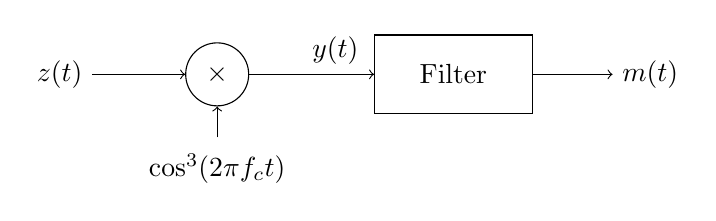
\begin{tikzpicture}
            % Nodes
            \node (z) at (0,0) {\( z(t) \)};
            \node [circle, draw, minimum size=0.8cm] (mult) at (2,0) {\(\times\)};
            \node [rectangle, draw, minimum width=2cm, minimum height=1cm] (filter) at (5,0) {Filter};
            \node (m) at (7.5,0) {\( m(t) \)};
            
            % Paths
            \draw[->] (z) -- (mult);
            \draw[->] (mult) -- (filter);
            \draw[->] (filter) -- (m);
            
            % Cosine multiplier
            \node at (2,-1.2) {\(\cos^3(2\pi f_c t)\)};
            \draw[->] (2,-0.8) -- (mult);
            
            % Labels
            \node at (3.5, 0.3) {\( y(t) \)};
        \end{tikzpicture}
    \end{center}

    We can recover the signal $m(t)$ by multiplying the received signal $z(t)$ by $\cos^3(2\pi f_c t)$ and passing it through a low pass filter with a cutoff frequency of $B$.
    \begin{align*}  
        Y(f) = \mathcal{F}\{y(t)\} &= \mathcal{F}\{z(t) \cos^3(2\pi f_c t)\} \\
        &= \mathcal{F}\{k m(t) \cos^4(2\pi f_c t)\}
    \end{align*}
    We know from 3.1 that $x(t) = m(t) \cos^3(2\pi f_c t)$, so we can write $y(t)$ as:
    \begin{align*}
        y(t) = k m(t) \cos^4(2\pi f_c t) = k x(t) \cos(2\pi f_c t)
    \end{align*}

    We can now modulate $X(f)$, which we found in 3.1, by $\cos(2\pi f_c t)$ to get $Y(f)$:
    \begin{align*}
        Y(f) &= kX(f) * \frac{1}{2} \left[\delta(f-f_c) + \delta(f+f_c)\right] \\
        &= \frac{k}{16} \left(
            \Lambda\left(\frac{f-3f_c}{B}\right) + 3\Lambda\left(\frac{f-f_c}{B}\right) + 3\Lambda\left(\frac{f+f_c}{B}\right) + \Lambda\left(\frac{f+3f_c}{B}\right) \ast \left[\delta(f-f_c) + \delta(f+f_c)\right]
        \right) \\ 
        &= \frac{k}{16}\Bigg(\Lambda\left(\frac{f-4f_c}{B}\right) + 3\Lambda\left(\frac{f-2f_c}{B}\right) + 3\Lambda\left(\frac{f}{B}\right) + \Lambda\left(\frac{f+2f_c}{B}\right) \\
            &+ \Lambda\left(\frac{f-2f_c}{B}\right) + 3\Lambda\left(\frac{f}{B}\right) + 3\Lambda\left(\frac{f+2f_c}{B}\right) + \Lambda\left(\frac{f+4f_c}{B}\right) \Bigg) \\
        &= \frac{k}{16}\Bigg(\Lambda\left(\frac{f-4f_c}{B}\right) + 4\Lambda\left(\frac{f-2f_c}{B}\right) + 6\Lambda\left(\frac{f}{B}\right) + 4\Lambda\left(\frac{f+2f_c}{B}\right) + \Lambda\left(\frac{f+4f_c}{B}\right) \Bigg)
    \end{align*}

    When we pass this through a filter with a cutoff frequency of $B$, we will get the message signal $m(t)$, scaled by a constant.
    \begin{align*}
        M(f) = Y(f)H(f) &= Y(f) \times \Pi\left(\frac{f}{B}\right) \\
        &= \frac{k}{16}\Lambda\left(\frac{f}{B}\right) \\
        \frac{k}{16}\Lambda\left(\frac{f}{B}\right) &\xrightarrow{\mathcal{F}^{-1}} \frac{kB}{16} \text{sinc}^2\left(Bt\right) = \frac{k}{16} m(t)
    \end{align*}
\end{enumerate}

% --------------------------------------------------------------------------------
% END BODY
% --------------------------------------------------------------------------------

\end{document}
ßf